\chapter{RESULTADOS E ANÁLISE}

Este capítulo apresenta os resultados dos experimentos conduzidos sobre o artefato descrito no Capítulo 4. A análise considera as métricas da Seção 2.8 e as questões de pesquisa QP1--QP4, com ênfase no desempenho comparativo (QP3) e nas limitações do ambiente de laboratório.

\section{Protocolo de coleta e ambiente}

As medições foram consolidadas a partir de arquivos JSON por execução em benchmarks/results/ agregados por npm run bench:agg em summary.csv e summary.json. Cada registro inclui tags de protocolo (h1, h2, h3), endpoint, carga (VUs), perfil de rede (network\_profile) e número de réplicas.

O conjunto de dados reportado neste capítulo compreende duas campanhas. A submatriz de rede degradada cobre GET /bench/ping, 50 VUs, quatro perfis de rede (clean, lag\_100ms, loss\_1pct, lag\_100ms\_loss\_1pct) e 10 réplicas por célula (12 células: três protocolos × quatro perfis), totalizando 120 execuções agregadas, com duração de 30 s e rampup de 5 s por execução, agregadas em benchmarks/results/2026-10-15\_10-13-06/. Já a matriz ideal cobre /bench/payload/:size (1 KB, 100 KB, 1 MB), POST /bench/echo (100 KB), GET /bench/ping com 10, 50 e 100 VUs, perfil clean apenas, 10 réplicas por célula (21 células, 210 execuções), com duração de 60 s e ramp-up de 10 s (Seção 5.4).

As duas campanhas foram executadas na mesma estação de trabalho com Windows 11 Pro (build 10.0.26200), processador AMD Ryzen 5 5600 com seis núcleos físicos e doze threads, cerca de 16 GB de RAM, arquitetura x86\_64. Ferramentas no host: k6 v2.2.0, Docker 29.4.2 e Node.js v22.13.0; API e NGINX em contêineres node:20-alpine na rede bench (docker-compose.bench.yml). Em ambas, k6 no host mediu HTTP/1.1 e HTTP/2, e o cliente QUIC (curl-http3 em contêiner) mediu HTTP/3, conforme benchmarks/README.md. A submatriz degradada não aplicou intervalo entre réplicas (cooldown\_sec = 0); a matriz ideal usou três minutos entre réplicas. Os p95 de /bench/ping com 50 VUs em clean nas duas campanhas são próximos (Seções 5.2 e 5.4), com diferença explicável pela duração do teste (30 s versus 60 s).

As cinco métricas da Seção 2.8 foram registradas em cada execução (http\_req\_duration para latência e tempo de resposta, http\_req\_waiting para TTFB, data\_received\_rate para taxa de transferência e http\_reqs\_rate para requisições por segundo). As tabelas principais deste capítulo destacam o percentil 95 de duração e a taxa de requisições; a Tabela 18 complementa a matriz ideal com TTFB e throughput de recepção agregados a partir do mesmo summary.csv. O cliente HTTP/3 não exporta data\_received\_rate no esquema normalizado, de modo que células correspondentes aparecem como ``---''.

\section{Submatriz degradada: perfil de controle (clean)}

Esta seção e a seguinte se referem exclusivamente à campanha de rede degradada (2026-10-15\_10-13-06), com 30 s por execução e sem intervalo entre réplicas. O perfil clean funciona como controle, sem netem; a matriz ideal, com variação de payload e de concorrência, é tratada separadamente na Seção 5.4.

A Tabela 11 resume a mediana do percentil 95 do tempo de requisição (http\_req\_duration\_p95, em milissegundos) e a mediana da taxa de requisições por segundo (http\_reqs\_rate), com dez réplicas por protocolo. Sob netem, o IQR entre réplicas no caminho HTTP/3 supera o de HTTP/1.1 e HTTP/2, o que é coerente com o uso de cliente QUIC em contêiner Docker (Seção 5.6)


\begin{table}[H]
\centering
\caption{Resultados - /bench/ping, 50 VUs, perfil clean da submatriz degradada (n = 10 réplicas)}
\small
\setlength{\tabcolsep}{3pt}
\begin{tabular}{@{}>{\raggedright\arraybackslash}p{42mm}>{\raggedright\arraybackslash}p{36mm}>{\raggedright\arraybackslash}p{32mm}>{\raggedright\arraybackslash}p{32mm}@{}} \hline
\textbf{Protocolo} & \textbf{p95 mediano (ms)} & \textbf{IQR p95 (ms)} & \textbf{req/s mediano} \\
\hline
HTTP/1.1 (direto) & 26,8 & 1,6 & 2203 \\
HTTP/2 (NGINX) & 32,5 & 1,3 & 1954 \\
HTTP/3 (NGINX QUIC) & 327,8 & 4,1 & 177 \\
\hline
\end{tabular}
\fonte{Fonte: elaborado pelo autor (agregação de benchmarks/results/2026-10-15\_10-13-06/summary.csv).}
\end{table}

Sem degradação de rede e com payload mínimo, HTTP/1.1 direto à API apresentou a menor latência no percentil 95 e a maior taxa de requisições entre os três caminhos. HTTP/2 via proxy ficou em posição intermediária, e HTTP/3 registrou p95 cerca de dez vezes maior que o de HTTP/2. Esse número não deve ser lido como desempenho intrínseco do protocolo sem considerar a ferramenta de carga (Seção 5.6). Os valores de /bench/ping com 50 VUs em clean ficam próximos aos da matriz ideal na mesma estação (28,5 ms, 34,3 ms e 351,7 ms para HTTP/1.1, HTTP/2 e HTTP/3, com 60 s por execução), o que indica consistência entre campanhas quando se compara o mesmo recorte (Seção 5.6).

\section{Rede degradada}

As Tabelas 12--14 apresentam o mesmo recorte (/bench/ping, 50 VUs, n = 10) para os perfis com tc netem. Sob latência artificial de 100 ms, os percentis 95 de HTTP/1.1 e HTTP/2 sobem para cerca de 112 ms e praticamente se igualam, enquanto HTTP/3 mantém valores mais altos, com IQR entre réplicas em torno de 11 ms em lag\_100ms.

No perfil loss\_1pct, HTTP/1.1 manteve p95 mediano equivalente ao clean (26,8 ms), HTTP/2 aumentou cerca de 5 ms (37,5 ms contra 32,5 ms) e HTTP/3 cerca de 18 ms (345,9 ms contra 327,8 ms). Com payload mínimo, a perda de 1\% no tráfego de saída teve efeito pequeno em HTTP/1.1 e efeito moderado nos caminhos via proxy e no cliente QUIC. HTTP/3 permaneceu na ordem de centenas de milissegundos.


\begin{table}[H]
\centering
\caption{Resultados --- perfil lag\_100ms (n = 10 réplicas)}
\small
\setlength{\tabcolsep}{3pt}
\begin{tabular}{@{}>{\raggedright\arraybackslash}p{28mm}>{\raggedright\arraybackslash}p{36mm}>{\raggedright\arraybackslash}p{32mm}>{\raggedright\arraybackslash}p{32mm}@{}} \hline
\textbf{Protocolo} & \textbf{p95 mediano (ms)} & \textbf{IQR p95 (ms)} & \textbf{req/s mediano} \\
\hline
HTTP/1.1 & 111,9 & 0,1 & 415 \\
HTTP/2 & 112,1 & 0,2 & 413 \\
HTTP/3 & 429,4 & 10,7 & 118 \\
\hline
\end{tabular}
\fonte{Fonte: elaborado pelo autor (agregação de benchmarks/results/2026-10-15\_10-13-06/summary.csv). }
\end{table}

\begin{table}[H]
\centering
\caption{Resultados --- perfil loss\_1pct (n = 10 réplicas)}
\small
\setlength{\tabcolsep}{3pt}
\begin{tabular}{@{}>{\raggedright\arraybackslash}p{28mm}>{\raggedright\arraybackslash}p{36mm}>{\raggedright\arraybackslash}p{32mm}>{\raggedright\arraybackslash}p{32mm}@{}} \hline
\textbf{Protocolo} & \textbf{p95 mediano (ms)} & \textbf{IQR p95 (ms)} & \textbf{req/s mediano} \\
\hline
HTTP/1.1 & 26,8 & 1,4 & 2199 \\
HTTP/2 & 37,5 & 0,8 & 1947 \\
HTTP/3 & 345,9 & 18,7 & 170 \\
\hline
\end{tabular}
\fonte{Fonte: elaborado pelo autor (agregação de benchmarks/results/2026-10-15\_10-13-06/summary.csv).}
\end{table}

\begin{table}[H]
\centering
\caption{Resultados --- perfil lag\_100ms\_loss\_1pct (n = 10 réplicas)}
\small
\setlength{\tabcolsep}{3pt}
\begin{tabular}{@{}>{\raggedright\arraybackslash}p{28mm}>{\raggedright\arraybackslash}p{36mm}>{\raggedright\arraybackslash}p{32mm}>{\raggedright\arraybackslash}p{32mm}@{}} \hline
\textbf{Protocolo} & \textbf{p95 mediano (ms)} & \textbf{IQR p95 (ms)} & \textbf{req/s mediano} \\
\hline
HTTP/1.1 & 110,8 & 0,1 & 396 \\
HTTP/2 & 111,0 & 0,2 & 396 \\
HTTP/3 & 458,3 & 13,5 & 114 \\
\hline
\end{tabular}
\fonte{Fonte: elaborado pelo autor (agregação de benchmarks/results/2026-10-15\_10-13-06/summary.csv).}
\end{table}

No perfil combinado lag\_100ms\_loss\_1pct, HTTP/1.1 e HTTP/2 seguem próximos entre si e praticamente iguais ao perfil lag\_100ms. HTTP/3 apresenta mediana de p95 superior à de lag\_100ms isolado (458,3 ms contra 429,4 ms), com IQR em torno de 14 ms, o que reforça a variabilidade do cliente QUIC sob perda e latência simultâneas. A literatura aponta que ganhos relativos de HTTP/3 dependem do contexto de rede e da carga (ZAHRA; ARDIANSYAH, 2026; TRIPATHI; MIRAZ; JOSHI, 2023), sem implicar superioridade universal.

A Figura 3 sintetiza visualmente o p95 mediano de duração por protocolo nos quatro perfis netem da submatriz degradada.

Na submatriz degradada, com /bench/ping e corpo de resposta mínimo, a mediana de http\_req\_waiting\_p95 praticamente coincide com a de http\_req\_duration\_p95 (diferença abaixo de 0,2 ms em k6; nula no cliente QUIC normalizado): com resposta tão pequena, o primeiro byte e o último chegam quase juntos. A Tabela 15 registra esse TTFB mediano (IQR) para completude.



\begin{figure}[H]
\centering
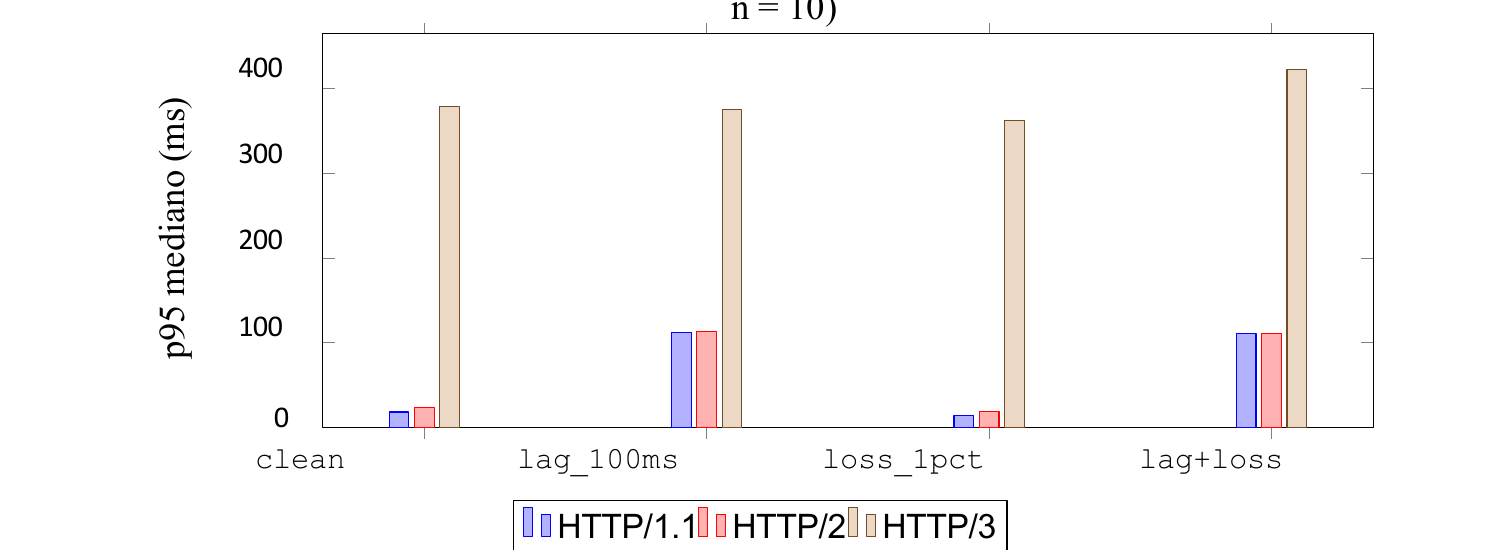
\includegraphics[width=0.92\textwidth]{assets/figuras/fig3.png}
\caption{Submatriz degradada - mediana do p95 de duração (/bench/ping, 50 VUs, n = 10)}
\fonte{Fonte: elaborado pelo autor (Tabelas 11--14).}
\end{figure}


\begin{table}[H]
\centering
\caption{Submatriz degradada - TTFB mediano (http\_req\_waiting\_p95), /bench/ping, 50 VUs (n = 10)}
\small
\setlength{\tabcolsep}{3pt}
\begin{tabular}{@{}>{\raggedright\arraybackslash}p{42mm}>{\raggedright\arraybackslash}p{32mm}>{\raggedright\arraybackslash}p{32mm}>{\raggedright\arraybackslash}p{32mm}@{}} \hline
\textbf{Perfil} & \textbf{HTTP/1.1} & \textbf{HTTP/2} & \textbf{HTTP/3} \\
\hline
clean & 26,7 (1,6) & 32,5 (1,3) & 327,8 (4,1) \\
lag\_100ms & 111,9 (0,1) & 112,1 (0,2) & 429,4 (10,7) \\
loss\_1pct & 26,7 (1,4) & 37,5 (0,8) & 345,9 (18,7) \\
lag\_\allowbreak 100ms\_\allowbreak loss\_\allowbreak 1pct & 110,8 (0,1) & 111 (0,2) & 458,3 (13,5) \\
\hline
\end{tabular}
\fonte{Fonte: elaborado pelo autor (benchmarks/results/2026-10-15\_10-13-06/summary.csv). Valores em milissegundos; entre parênteses, IQR entre réplicas. Em /bench/ping, TTFB e p95 de duração diferem menos de 0,2 ms em k6 e coincidem no cliente QUIC}
\end{table}

\section{Variação de payload e níveis de concorrência}

A matriz de payload e de concorrência em rede ideal (clean) foi executada conforme o desenho do Capítulo 4: GET /bench/ping com 10, 50 e 100 VUs; GET /bench/payload/:size (1 KB, 100 KB e 1 MB) e POST /bench/echo (corpo de 100 KB) com 50 VUs; três protocolos por célula; 60 s de duração e ramp-up de 10 s; 10 réplicas por célula (21 células, 210 execuções), com intervalo de três minutos entre réplicas. A campanha foi agregada em benchmarks/results/2026-10-01\_08-38-06/, e todas as execuções registraram http\_req\_failed\_rate nulo. O ambiente de coleta é o mesmo da submatriz degradada (Seção 5.1); diferem a duração do teste, o intervalo entre réplicas e o desenho experimental.

A Tabela 16 resume a variação de concorrência em /bench/ping. A Tabela 17 resume payload e echo com carga fixa de 50 VUs. Em ambas, reportam-se a mediana do percentil 95 do tempo de requisição, o IQR entre réplicas e a mediana da taxa de requisições por segundo, no mesmo formato das demais tabelas deste capítulo.


\begin{table}[H]
\centering
\caption{Matriz ideal - /bench/ping, perfil clean (n = 10 réplicas)}
\small
\setlength{\tabcolsep}{3pt}
\begin{tabular}{@{}>{\raggedright\arraybackslash}p{12mm}>{\raggedright\arraybackslash}p{40mm}>{\raggedright\arraybackslash}p{34mm}>{\raggedright\arraybackslash}p{28mm}>{\raggedright\arraybackslash}p{26mm}@{}} \hline
\textbf{VUs} & \textbf{Protocolo} & \textbf{p95 mediano (ms)} & \textbf{IQR p95 (ms)} & \textbf{req/s mediano} \\
\hline
10 & HTTP/1.1 (direto) & 7,5 & 0,1 & 2200 \\
10 & HTTP/2 (NGINX) & 8,6 & 0,5 & 1856 \\
10 & HTTP/3 (NGINX QUIC) & 58,9 & 1,5 & 163 \\
50 & HTTP/1.1 (direto) & 28,5 & 1,2 & 2240 \\
50 & HTTP/2 (NGINX) & 34,3 & 1,8 & 1908 \\
50 & HTTP/3 (NGINX QUIC) & 351,7 & 24,0 & 180 \\
100 & HTTP/1.1 (direto) & 51,4 & 3,6 & 2178 \\
100 & HTTP/2 (NGINX) & 60,0 & 2,1 & 1877 \\
100 & HTTP/3 (NGINX QUIC) & 699,3 & 30,0 & 186 \\
\hline
\end{tabular}
\fonte{Fonte: elaborado pelo autor (agregação de benchmarks/results/2026-10-01\_08-38-06/summary.csv).}
\end{table}



\begin{table}[H]
\centering
\caption{Matriz ideal - payload e echo, 50 VUs, perfil clean (n = 10 réplicas)}
\footnotesize
\setlength{\tabcolsep}{2.5pt}
\begin{tabular}{@{}>{\raggedright\arraybackslash}p{30mm}>{\raggedright\arraybackslash}p{38mm}>{\raggedright\arraybackslash}p{32mm}>{\raggedright\arraybackslash}p{22mm}>{\raggedright\arraybackslash}p{20mm}@{}} \hline
\textbf{Cenário} & \textbf{Protocolo} & \textbf{p95 mediano (ms)} & \textbf{IQR p95 (ms)} & \textbf{req/s mediano} \\
\hline
GET 1 KB & HTTP/1.1 (direto) & 29,4 & 1,8 & 2189 \\
GET 1 KB & HTTP/2 (NGINX) & 36,4 & 0,7 & 1843 \\
GET 1 KB & HTTP/3 (NGINX QUIC) & 342,5 & 14,6 & 183 \\
GET 100 KB & HTTP/1.1 (direto) & 50,8 & 3,0 & 1468 \\
GET 100 KB & HTTP/2 (NGINX) & 81,3 & 2,3 & 1041 \\
GET 100 KB & HTTP/3 (NGINX QUIC) & 563,5 & 34,2 & 112 \\
GET 1 MB & HTTP/1.1 (direto) & 232,6 & 15,1 & 241 \\
GET 1 MB & HTTP/2 (NGINX) & 325,9 & 10,3 & 178 \\
GET 1 MB & HTTP/3 (NGINX QUIC) & 2779,6 & 170,9 & 19 \\
POST echo 100 KB & HTTP/1.1 (direto) & 50,9 & 2,6 & 1192 \\
POST echo 100 KB & HTTP/2 (NGINX) & 91,1 & 3,1 & 924 \\
POST echo 100 KB & HTTP/3 (NGINX QUIC) & 1542,4 & 61,8 & 81 \\
\hline
\end{tabular}
\fonte{Fonte: elaborado pelo autor (agregação de benchmarks/results/2026-10-01\_08-38-06/summary.csv).}
\end{table}


A Figura 4 ilustra o crescimento do p95 mediano em /bench/ping conforme a concorrência na matriz ideal.

\begin{figure}[H]
\centering
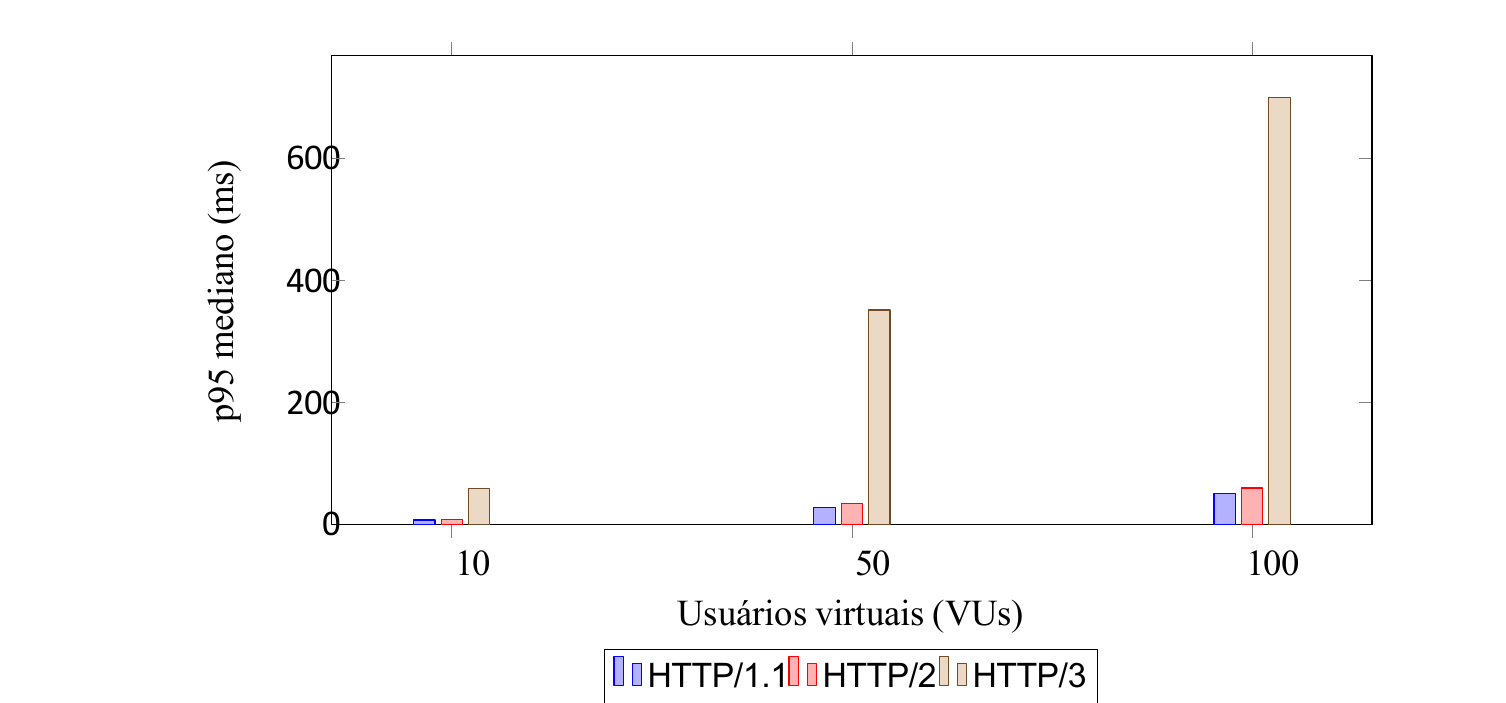
\includegraphics[width=0.92\textwidth]{assets/figuras/fig4.png}
\caption{Matriz ideal - mediana do p95 de duração em /bench/ping por nível de concorrência (n = 10)}
\fonte{Fonte: elaborado pelo autor (Tabela 16).}
\end{figure}

A Tabela 18 reporta TTFB (http\_req\_waiting\_p95) e taxa de recepção (data\_received\_rate) na mesma campanha. Em transferências volumosas (GET 1 MB), o TTFB permanece baixo em HTTP/1.1 e HTTP/2 enquanto o tempo total de resposta cresce (Tabela 17), separando o custo de estabelecimento e início de resposta do tempo de transferência do corpo.

Na matriz ideal, HTTP/1.1 direto à API registrou menores p95 e maiores taxas de requisição que os caminhos via NGINX; entre HTTP/2 e HTTP/3 no mesmo proxy, HTTP/2 apresentou p95 mais baixo e taxa de requisições mais alta em todas as células. A latência cresce com a concorrência e com o tamanho do corpo, e a distância entre HTTP/3 e os demais aumenta em transferências volumosas (p95 mediano de 2779,6 ms no GET de 1 MB). Essas diferenças devem ser lidas à luz da assimetria de topologia e do cliente QUIC (Seção 5.6); a interpretação detalhada consta na Seção 5.5.


\begin{table}[H]
\centering
\caption{Matriz ideal - TTFB e throughput de recepção (n = 10 réplicas, campanha 2026-10-01\_08-38-06)}
\footnotesize
\setlength{\tabcolsep}{2.5pt}
\begin{tabular}{@{}>{\raggedright\arraybackslash}p{34mm}>{\raggedright\arraybackslash}p{22mm}>{\raggedright\arraybackslash}p{28mm}>{\raggedright\arraybackslash}p{18mm}>{\raggedright\arraybackslash}p{28mm}@{}} \hline
\textbf{Cenário} & \textbf{Protocolo} & \textbf{TTFB p95 (ms)} & \textbf{IQR (ms)} & \textbf{Recepção} \\
\hline
\textit{/bench/ping} &  &  &  &  \\
10 VUs & HTTP/1.1 & 7,5 & 0,2 & 2084 KB/s \\
10 VUs & HTTP/2 & 8,6 & 0,5 & 1331 KB/s \\
10 VUs & HTTP/3 & 58,9 & 1,5 & --- \\
50 VUs & HTTP/1.1 & 28,5 & 1,2 & 2122 KB/s \\
50 VUs & HTTP/2 & 34,2 & 1,9 & 1369 KB/s \\
50 VUs & HTTP/3 & 351,7 & 24,0 & --- \\
100 VUs & HTTP/1.1 & 51,4 & 3,6 & 2063 KB/s \\
100 VUs & HTTP/2 & 59,8 & 2,2 & 1348 KB/s \\
100 VUs & HTTP/3 & 699,3 & 30,0 & --- \\
GET 1 KB & HTTP/1.1 & 29,4 & 1,8 & 4,04 MB/s \\
GET 1 KB & HTTP/2 & 36,3 & 0,6 & 3,01 MB/s \\
GET 1 KB & HTTP/3 & 342,5 & 14,6 & --- \\
GET 100 KB & HTTP/1.1 & 50,2 & 2,9 & 144,69 MB/s \\
GET 100 KB & HTTP/2 & 79,7 & 2,8 & 102,69 MB/s \\
GET 100 KB & HTTP/3 & 563,5 & 34,2 & --- \\
GET 1 MB & HTTP/1.1 & 20,5 & 1,8 & 241,67 MB/s \\
GET 1 MB & HTTP/2 & 36,7 & 1,4 & 179,25 MB/s \\
GET 1 MB & HTTP/3 & 2779,6 & 170,9 & --- \\
POST echo 100 KB & HTTP/1.1 & 50,6 & 2,6 & 1,11 MB/s \\
POST echo 100 KB & HTTP/2 & 88,4 & 2,8 & 0,69 MB/s \\
POST echo 100 KB & HTTP/3 & 1542,4 & 61,8 & --- \\
\hline
\end{tabular}
\fonte{Fonte: elaborado pelo autor (benchmarks/results/2026-10-01\_08-38-06/summary.csv). Recepção: mediana de data\_received\_rate (k6); ``---'' indica métrica não exportada pelo cliente HTTP/3.}
\end{table}

\section{Análise e discussão}

Acerca da viabilidade e integração (QP1 e QP4), as campanhas em rede clean e degradada mostram que o caminho HTTP/3 permaneceu operacional, com taxa de falha nula em todas as células agregadas. O artefato (API, NGINX, Docker e runners) foi executado com o mesmo roteiro na mesma estação, em duas campanhas independentes, o que indica reprodutibilidade operacional no ambiente de laboratório, embora não substitua replicação em outro hardware. A estratégia de proxy reverso materializa uma migração incremental sem alterar o backend Node.js, alinhada a estudos com integração de proxy (MUÑOZ et al., 2025).

 Três limites estruturais condicionam a leitura dos números para análise do desempenho comparativo (QP3) e viés de desenho. Primeiro, HTTP/1.1 foi medido com acesso direto à API (:3000), enquanto HTTP/2 e HTTP/3 passam pelo NGINX (:8443); portanto, posicionar HTTP/1.1 como ``melhor protocolo'' confunde efeito de topologia com efeito de versão HTTP. A comparação menos enviesada no laboratório é entre HTTP/2 e HTTP/3, ambos terminados no mesmo proxy; mesmo assim, o HTTP/3 registrou p95 mais alto e taxa de requisições mais baixa em todas as tabelas reportadas (Tabelas 16, 17 e 18; Figuras 3 e 4).

Segundo, o p95 mediano de HTTP/3 em /bench/ping com 50 VUs permaneceu na ordem de centenas de milissegundos em clean (327,8 ms na campanha degradada; 351,7 ms na matriz ideal). Sob lag\_100ms, o p95 de HTTP/3 sobe cerca de 102 ms (429,4 ms), incremento semelhante ao de HTTP/1.1 e HTTP/2 (cerca de 85 ms), mas somado a uma base já alta, dominada pelo cliente QUIC em contêiner. Na matriz ideal, enquanto a concorrência sobe de 10 para 100 VUs, a taxa de requisições de HTTP/3 fica praticamente estável (163, 180 e 186 req/s) e o p95 cresce quase na mesma proporção dos VUs (58,9, 351,7 e 699,3 ms), comportamento típico de um teto de vazão em que as requisições adicionais apenas esperam na fila. Esse padrão sugere que a ordem de grandeza observada para HTTP/3 é determinada sobretudo pelo cliente QUIC em contêiner e pelo pipeline de medição; o efeito de rede simulado modula o valor absoluto, mas não altera a distância em relação a HTTP/1.1 e HTTP/2 medidos com k6.

Terceiro, na matriz ideal o TTFB reportado para HTTP/3 coincide com o tempo total de resposta em /bench/ping e em transferências volumosas (por exemplo, 2779,6 ms no GET de 1 MB), enquanto HTTP/1.1 e HTTP/2 exibem TTFB baixo com duração total maior (Tabela 18). Assim, métricas homônimas entre k6 e o cliente QUIC não são diretamente comparáveis. Diante desses limites, os dados não permitem concluir superioridade ou inferioridade intrínseca de HTTP/3; apenas registram o comportamento fim a fim (\textit{end-to-end}) do arranjo medido, em linha com evidências contextuais da literatura (ZAHRA; ARDIANSYAH, 2026; PERNA et al., 2022; TRIPATHI; MIRAZ; JOSHI, 2023; ZHANG et al., 2025).

Os resultados informam mais a decisão sobre como expor HTTP/3 (proxy, certificados, UDP, observabilidade) do que sobre quando HTTP/3 supera HTTP/2. A integração por proxy introduz custos operacionais discutidos na literatura (MUÑOZ et al., 2025; TRIPATHI; MIRAZ; JOSHI, 2023), e interpretar a latência fim a fim exige correlacionar ferramentas de carga, logs do NGINX e Server-Timing (Capítulo 4), tarefa que fica como continuidade empírica.

\section{Ameaças à validade e limitações}

A submatriz degradada restringiu-se a GET /bench/ping com 50 VUs e quatro perfis netem (Seções 5.2 e 5.3). A matriz ideal avaliou payload (1 KB, 100 KB, 1 MB), POST /bench/echo e concorrência (10, 50 e 100 VUs) apenas em rede clean (Seção 5.4), sem combinar essas dimensões com netem. Combinações completas de payload e concorrência sob todos os perfis degradados permanecem fora do escopo quantitativo deste trabalho.

A submatriz degradada e a matriz ideal foram executadas na mesma estação (Seção 5.1), sem replicação em outro hardware ou sistema operacional, o que limita a generalização dos achados para outros ambientes de coleta. As comparações dentro de cada campanha devem ser lidas nesse contexto; diferenças pontuais entre campanhas podem refletir duração do teste e intervalo entre réplicas, além dos protocolos ou cenários.

Nota-se, também, uma assimetria topológica no experimento, visto que o HTTP/1.1 foi exercitado sem NGINX, enquanto HTTP/2 e HTTP/3 compartilham terminação TLS/QUIC na borda. Comparações que incluem HTTP/1.1 direto misturam efeito de proxy com efeito de protocolo.

Diferentemente de HTTP/1.1 e HTTP/2 (k6), HTTP/3 foi medido por cliente QUIC em Docker, com menor paralelismo efetivo e maior variabilidade entre réplicas sob \textit{nete}\textit{m} (IQR de p95 entre cerca de 11 ms e 19 ms nos perfis degradados da submatriz, contra menos de 0,2 ms em HTTP/1.1 e HTTP/2 em \textit{lag\_100ms}). A taxa de requisições de HTTP/3 não acompanha o aumento de VUs na matriz ideal, reforçando que o gerador limita a medida. Assim, comparações diretas de  \textit{throughput} e latência entre h3 e h1/h2 tendem a distorcer a avaliação do QUIC em relação ao que um gerador de carga homogêneo mostraria. Essa limitação está documentada no repositório do artefato.

Por fim, testes em localhost ou rede Docker não reproduzem a Internet pública; o netem aproxima, mas não substitui, condições de operadoras e middleboxes.

